\chapter{Analyses Hive SQL et Spark SQL}
% Pour chaque analyse : question -> tables -> requête -> résultat -> interprétation.

\section{Jointure offres $\leftrightarrow$ metiers}

\textbf{Question} : quels sont les métiers avec le plus d'offres et
leur salaire moyen associé ?

\textbf{Requête} (Hive SQL, exécutée via Beeline) :

\begin{verbatim}
SELECT m.job_title, COUNT(*) AS n,
       ROUND(AVG(o.annual_salary_usd),0) AS avg_sal
FROM processed.offres o
JOIN processed.metiers m ON o.metier_id = m.metier_id
GROUP BY m.job_title
ORDER BY n DESC
LIMIT 5;
\end{verbatim}

\textbf{Résultat} :

\begin{center}
\begin{tabular}{lrr}
\toprule
Métier & Offres & Salaire moyen (\$) \\
\midrule
LLM Engineer & 75 & 240\,960 \\
Robotics Engineer (AI) & 74 & 170\,851 \\
Prompt Engineer & 71 & 151\,451 \\
Generative AI Engineer & 71 & 206\,761 \\
AI Product Manager & 70 & 194\,571 \\
\bottomrule
\end{tabular}
\end{center}

\begin{constat}[Interprétation]
La jointure \texttt{offres} $\leftrightarrow$ \texttt{metiers} via
\texttt{metier\_id} fonctionne correctement de bout en bout (HDFS
Parquet $\to$ tables Hive externes $\to$ requête SQL avec jointure et
agrégation). \textbf{LLM Engineer} arrive en tête à la fois en volume
(75 offres, le plus demandé du dataset) et en rémunération (240\,960\$
en moyenne, largement au-dessus des autres métiers du top 5), ce qui
est cohérent avec la prime salariale généralement associée aux
compétences LLM/GenAI observée par ailleurs dans le dataset
(\texttt{ai\_salary\_premium\_pct}, \texttt{is\_llm\_role}).
\end{constat}

\section{Jointure offres $\leftrightarrow$ competences}

\textbf{Question} : quelles compétences sont associées au plus grand
nombre d'offres, et à quel salaire moyen ?

\textbf{Requête} (exécutée via Beeline) :

\begin{verbatim}
SELECT c.competence, COUNT(DISTINCT o.job_id) AS nb_offres,
       ROUND(AVG(o.annual_salary_usd), 0) AS salaire_moyen
FROM processed.offres o
JOIN processed.competences c ON o.job_id = c.job_id
GROUP BY c.competence
ORDER BY nb_offres DESC, c.competence ASC
LIMIT 10;
\end{verbatim}

\textbf{Résultat} :

\begin{center}
\begin{tabular}{lrr}
\toprule
Compétence & Offres & Salaire moyen (\$) \\
\midrule
Python & 942 & 197\,500 \\
SQL & 422 & 188\,921 \\
Cloud & 402 & 198\,644 \\
Communication & 365 & 184\,460 \\
Leadership & 363 & 199\,056 \\
\bottomrule
\end{tabular}
\end{center}

\begin{constat}[Méthode de comptage]
Le nombre d'offres est calculé avec \texttt{COUNT(DISTINCT job\_id)}
pour éviter toute inflation liée à d'éventuelles répétitions de
compétences dans \texttt{required\_skills}. La moyenne salariale
(\texttt{AVG}) porte sur toutes les lignes jointes, ce qui rend le
dédoublonnage de la table \texttt{competences} indispensable pour ne
pas compter plusieurs fois le salaire d'une même offre. Après
dédoublonnage, les écarts de salaire moyen restent inférieurs à 2\,\%
sans changement de classement.
\end{constat}

\begin{figure}[h]
\centering
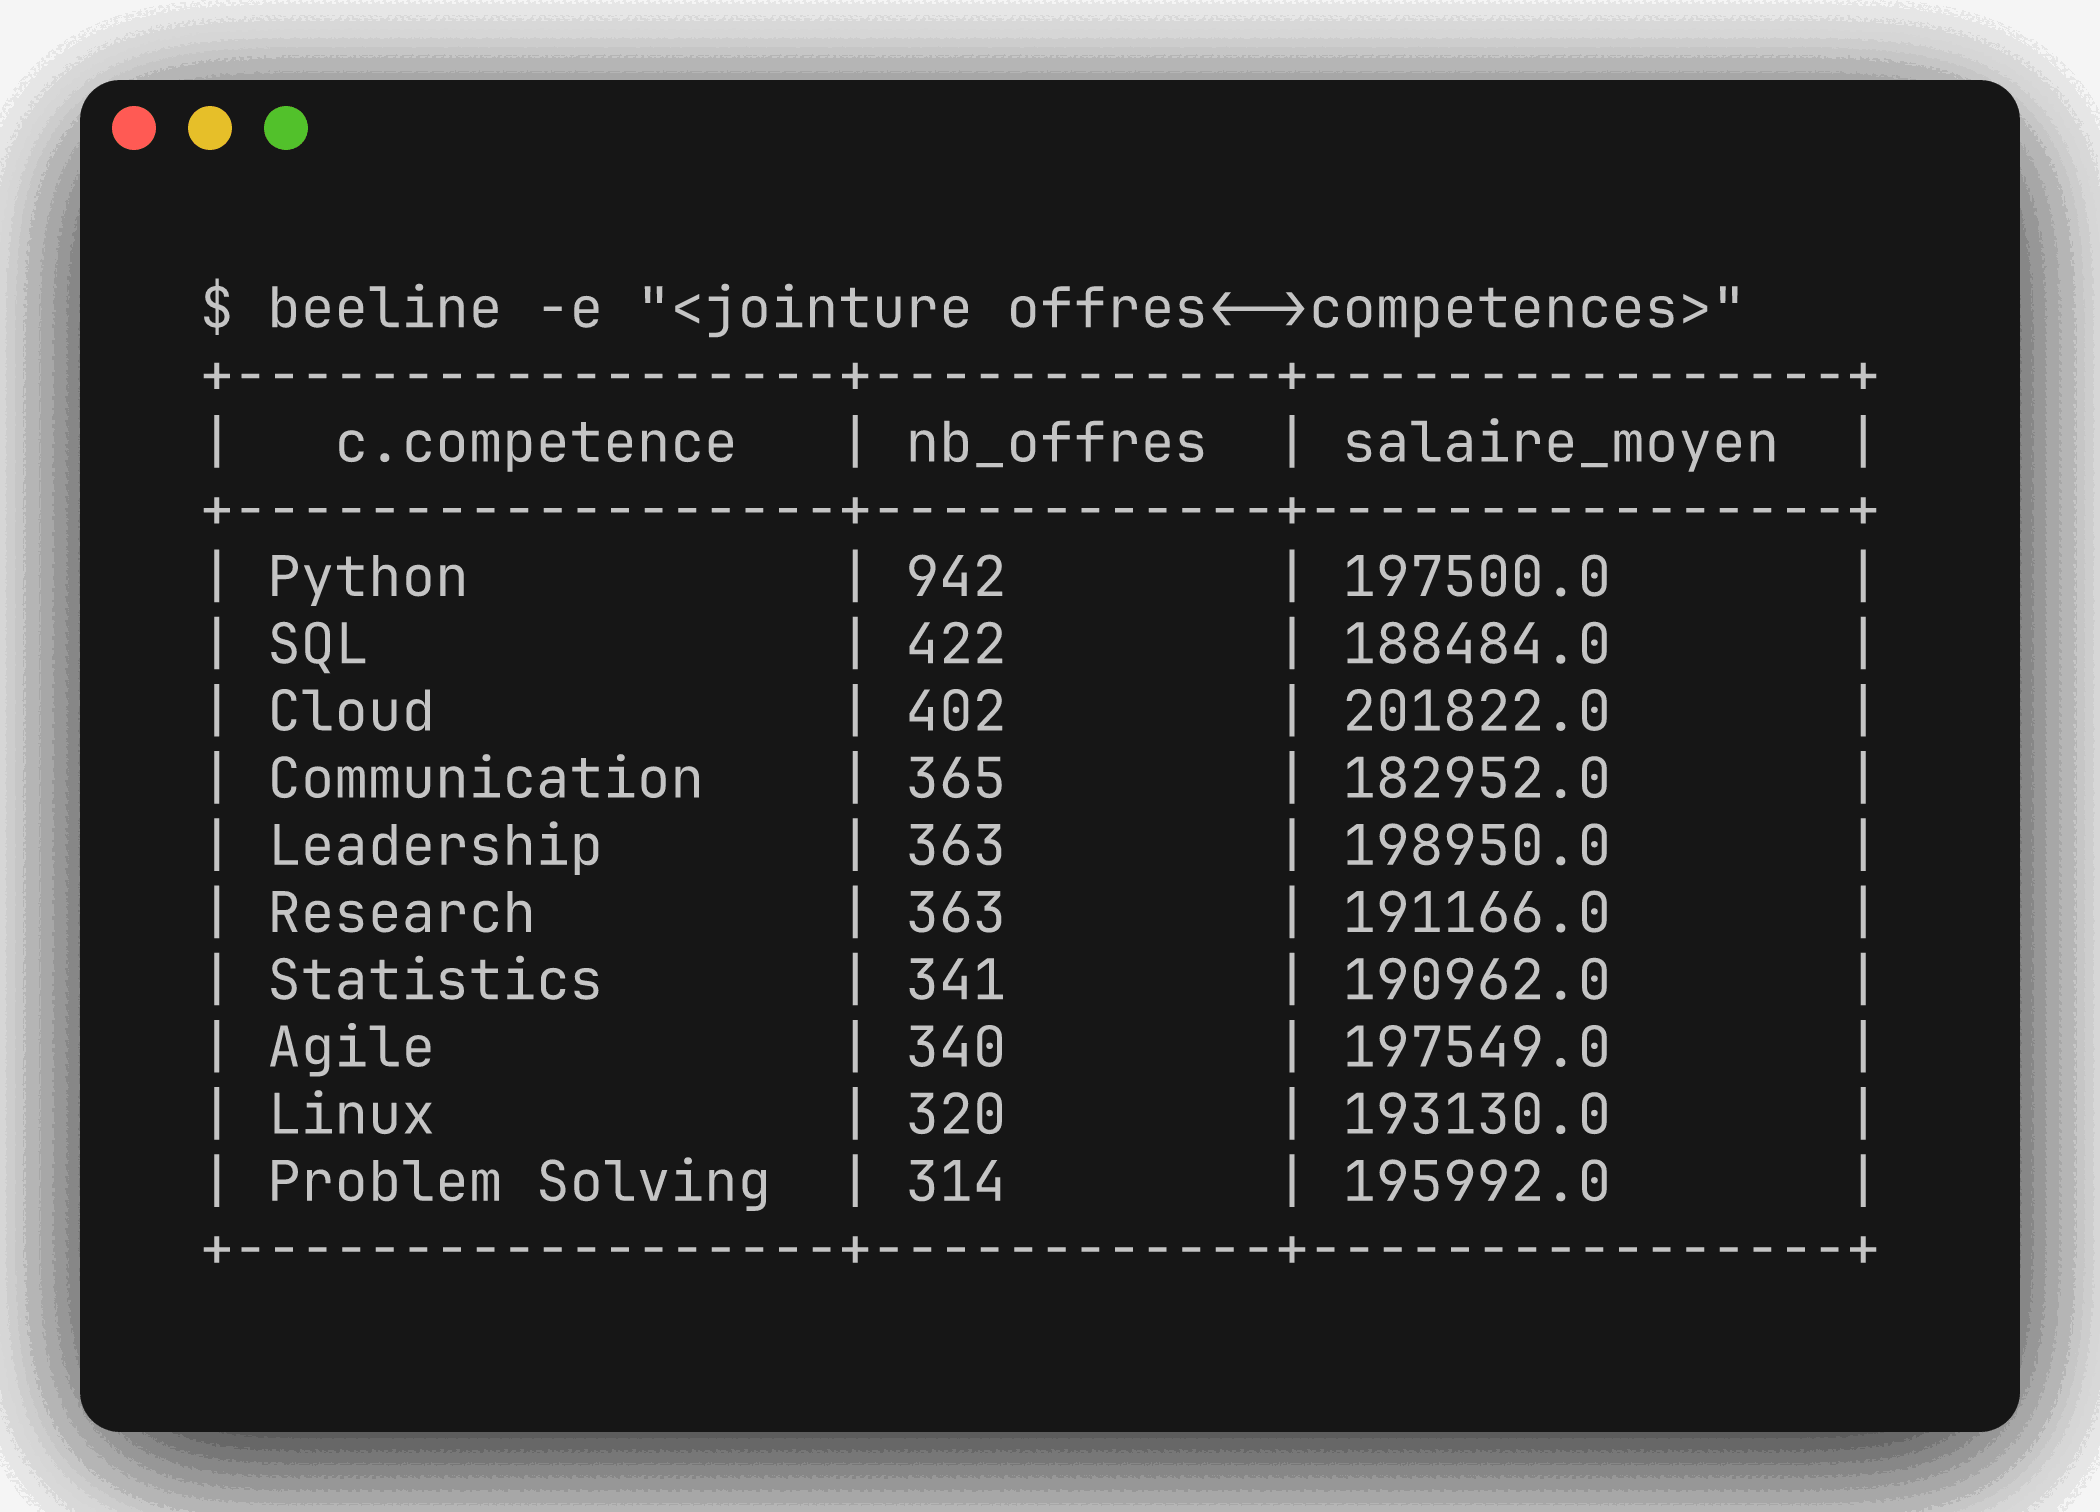
\includegraphics[width=0.85\linewidth]{figures/etape3_join_offres_competences.png}
\caption{Jointure \texttt{offres}$\leftrightarrow$\texttt{competences}
via Beeline.}
\end{figure}

\begin{constat}[Interprétation]
Python apparaît dans 942 des 1500 offres (63\,\%), largement devant
toute autre compétence, ce qui est cohérent avec son statut de socle
universel du poste IA, indépendamment du métier précis. Les compétences techniques
(SQL, Cloud) et non techniques (Communication, Leadership) se
mélangent dans le top 10, signe que les postes IA valorisés dans ce
dataset ne sont pas uniquement des postes techniques « pures ».
\end{constat}

\section{Requête GROUP BY + HAVING}

\textbf{Question} : quels pays combinent un volume d'offres important
(> 50) et une rémunération moyenne élevée (> 150\,000\$) ?

\begin{verbatim}
SELECT country, COUNT(*) AS nb_offres,
       ROUND(AVG(annual_salary_usd), 0) AS salaire_moyen
FROM processed.offres
GROUP BY country
HAVING COUNT(*) > 50 AND AVG(annual_salary_usd) > 150000
ORDER BY salaire_moyen DESC;
\end{verbatim}

\textbf{Résultat} : 12 pays satisfont les deux conditions, de
\textbf{USA} (515 offres, 226\,190\$ en moyenne) à \textbf{Japon}
(76 offres, 170\,132\$). Les États-Unis dominent à la fois en volume
(plus du tiers des offres du dataset) et en rémunération moyenne du
top 12.

\begin{figure}[h]
\centering
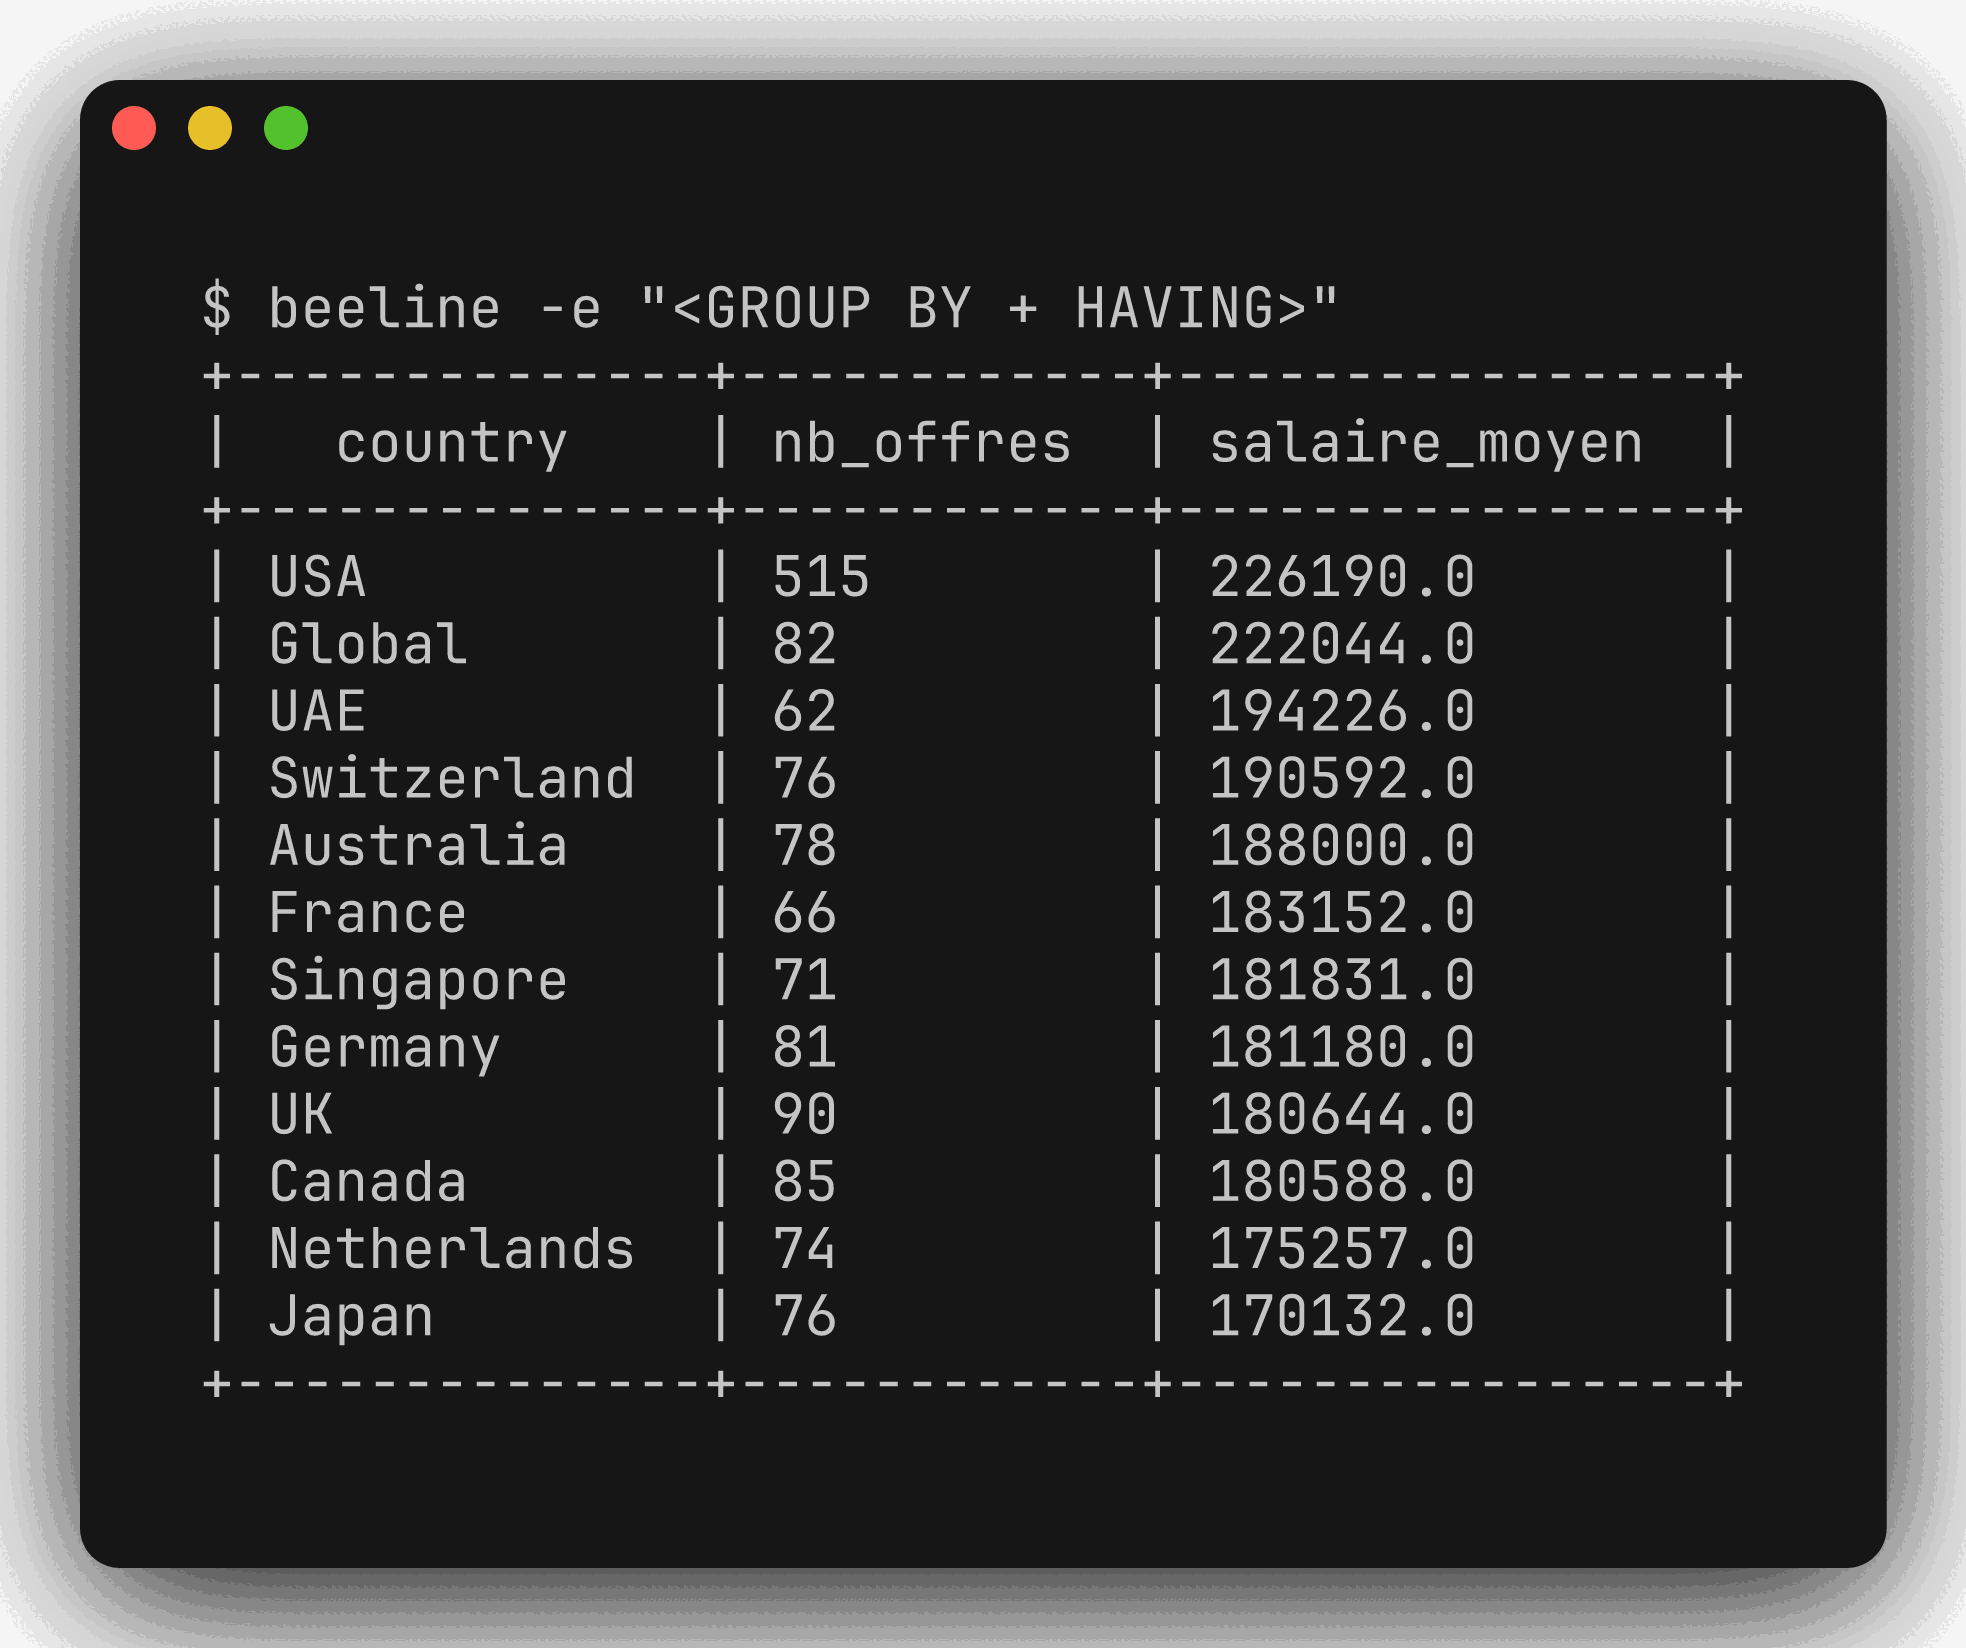
\includegraphics[width=0.85\linewidth]{figures/etape3_group_by_having.png}
\caption{Requête \texttt{GROUP BY} + \texttt{HAVING} via Beeline.}
\end{figure}

\section{Hive SQL vs Spark SQL : même requête, deux moteurs}

\textbf{Requête} (identique dans les deux cas) : salaire moyen par
niveau d'expérience. Elle porte sur la table
\texttt{processed.offres}.

\begin{center}
\begin{tabular}{lrr}
\toprule
Niveau d'expérience & Offres & Salaire moyen (\$) \\
\midrule
Lead (10+ yrs) & 381 & 240\,055 \\
Senior (6-9 yrs) & 364 & 214\,280 \\
Mid (3-5 yrs) & 370 & 175\,984 \\
Entry (0-2 yrs) & 385 & 150\,039 \\
\bottomrule
\end{tabular}
\end{center}

\begin{figure}[h]
\centering
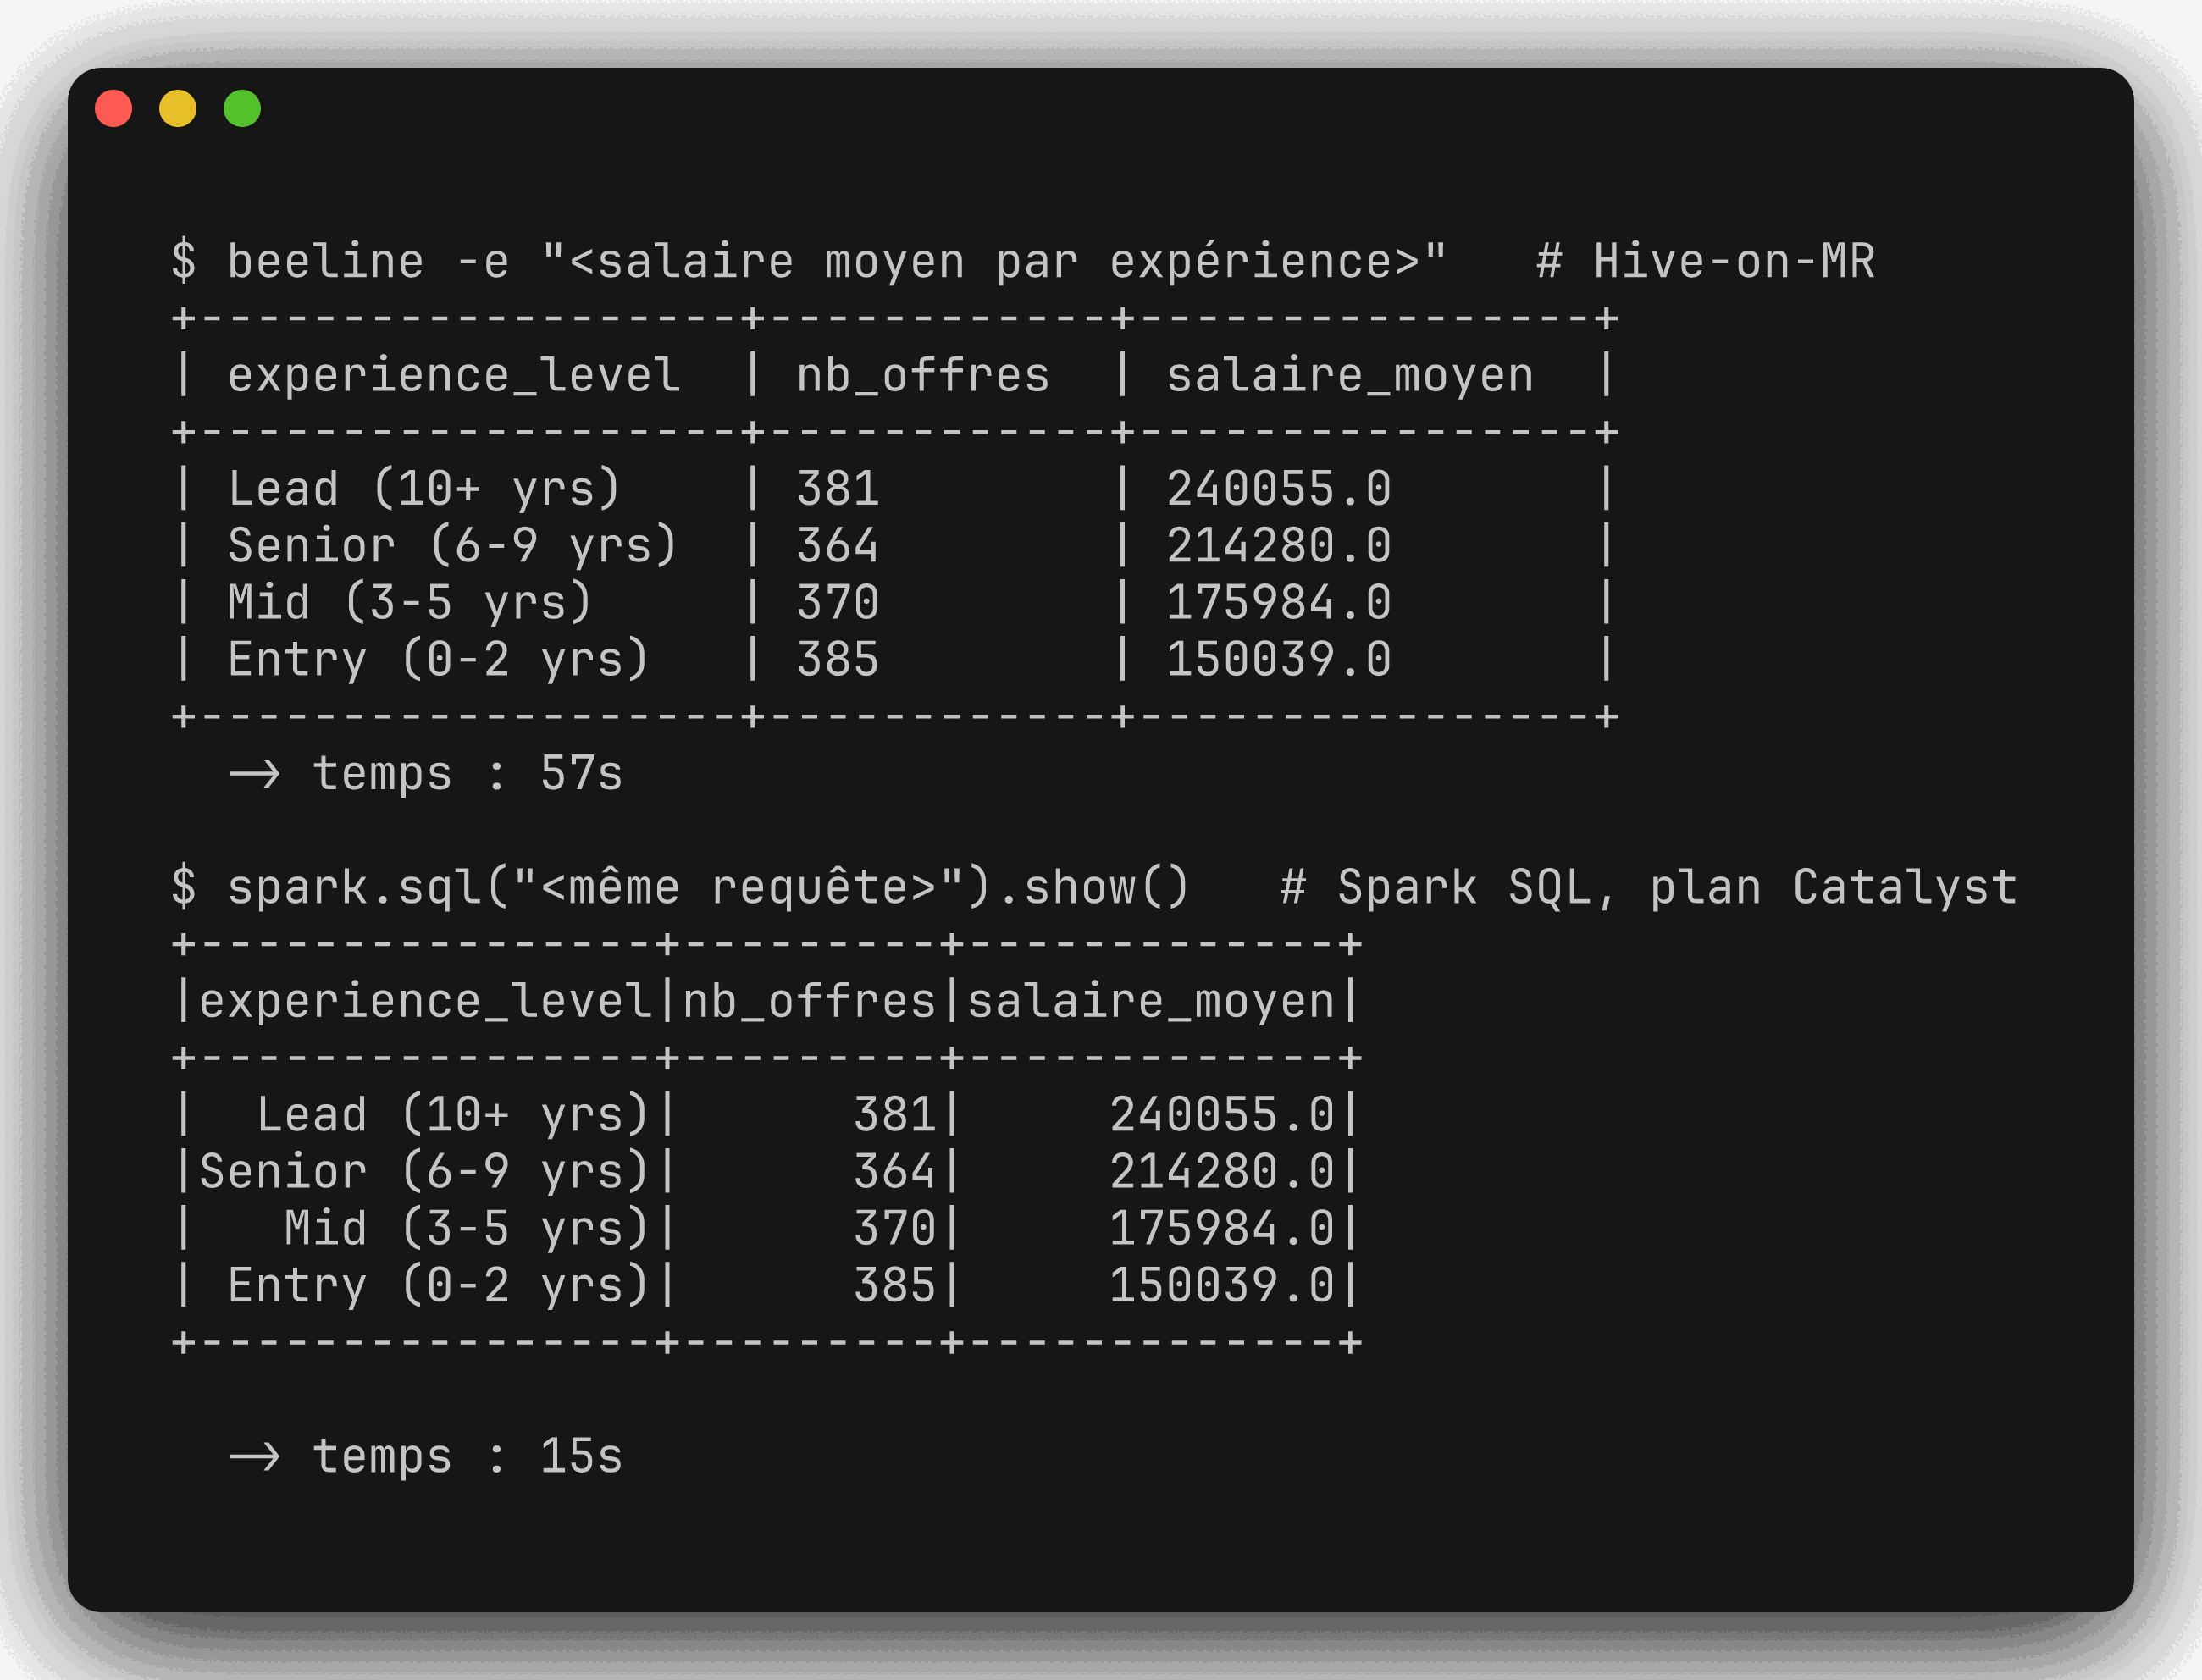
\includegraphics[width=0.85\linewidth]{figures/etape3_hive_vs_spark_sql.png}
\caption{Même requête exécutée via Beeline (Hive-on-MR) puis
\texttt{spark.sql(...)} (Spark SQL), avec les temps mesurés sur ce run.}
\end{figure}

\begin{constat}[Interprétation]
Les deux moteurs renvoient exactement le même résultat, comme attendu
(même source de données, même sémantique SQL), mais avec un écart de
temps d'exécution notable sur cette machine :

\begin{itemize}[leftmargin=1.5em]
  \item \textbf{Hive SQL} (Beeline, moteur Hive-on-MR) : 57 secondes.
  \item \textbf{Spark SQL} (\texttt{spark.sql(...)} depuis Jupyter) :
    15 secondes, SparkSession déjà chaude comprise.
\end{itemize}

L'écart qualitatif est systématique : Spark SQL est nettement plus
rapide, dans un rapport de 3 à 4$\times$. Hive-on-MR matérialise des
étapes MapReduce sur disque, alors que Spark SQL exécute un plan
Catalyst optimisé en mémoire. C'est une illustration chiffrée, sur ce
dataset, de l'intérêt de Spark pour l'analytique interactive, Hive
restant utilisé comme couche de métadonnées et de requêtage SQL
classique.
\end{constat}
